\documentclass[journal,12pt,twocolumn]{IEEEtran}
\usepackage{amsmath,amssymb,amsfonts,amsthm}
\usepackage{txfonts}
\usepackage{tkz-euclide}
\usepackage{listings}
\usepackage{gvv}
\usepackage[latin1]{inputenc}
\usepackage{array}
\usepackage{pgf}
\usepackage{lmodern}

\begin{document}
\bibliographystyle{IEEEtran}

\vspace{3cm}

\title{}
\author{EE23BTECH11054 -  Sai Krishna Shanigarapu$^{*}$
}
\maketitle
\newpage
\bigskip

% \renewcommand{\thefigure}{\theenumi}
% \renewcommand{\thetable}{\theenumi}

\section*{Exercise 9.2}

\noindent \textbf{13} \hspace{2pt}If the sum of $n$ terms of an A.P. is $3n^2+5n$ and its $m^{th}$ term is 164, find the value of $m$.
\bigskip

\solution:
\noindent
\begin{align}
Y \brak{z} &= \frac{2z^2\brak{4z-1}}{\brak{z-1}^3} & \cbrak{z\in\mathbb{C} : |z| > 1}\\
U\brak{z} &= \frac{1}{1-z^{-1}} & \cbrak{z\in\mathbb{C} : |z| > 1}\\
%y\brak{n} &= x\brak{n}*u\brak{n}\\
X\brak{z} &=  \frac{Y\brak{z}}{U\brak{z}}\\
%&= 2\left(\frac{z}{z-1}\right) + 6\left(\frac{z}{z-1}\right) ^2\\
x\brak{n} &= Z_{z}^{-1}\left[2\left(\frac{z}{z-1}\right) + 6\left(\frac{z}{z-1}\right) ^2\right]\\
%&= 2\brak{u\brak{n}} + 6\brak{n+1}\brak{u\brak{n}}\\
&= \brak{6n+8}\brak{u\brak{n}}
\end{align}

\begin{figure}[h]
    \centering
    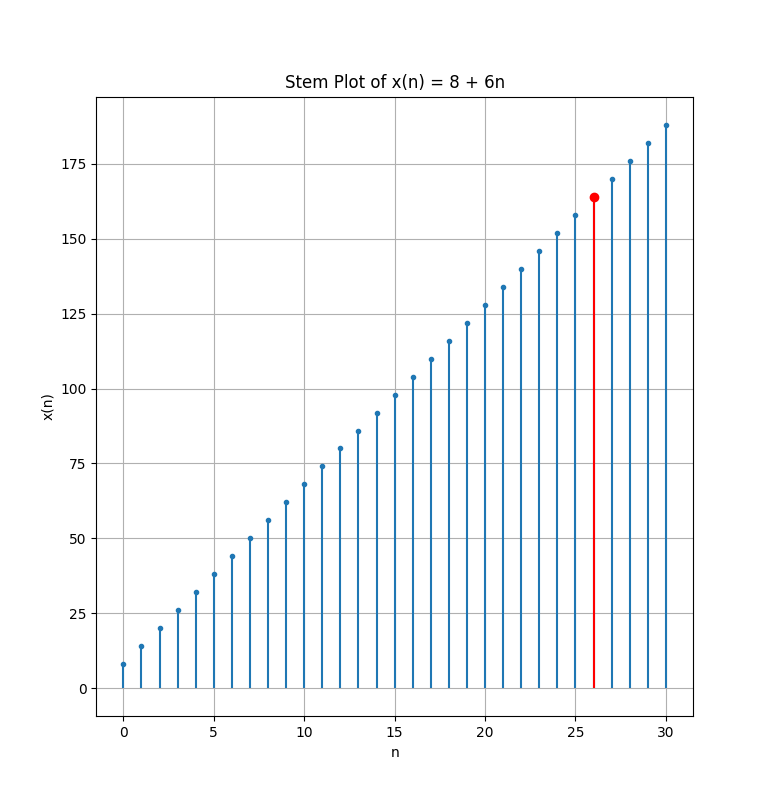
\includegraphics[width=1\columnwidth]{figs/Figure_1.png}
    \caption{Plot of x(n) vs n}
    \label{fig:11.9.2.13.1}
\end{figure}
    $\therefore m$ = 26
    
\setlength{\arrayrulewidth}{0.3mm}
\setlength{\tabcolsep}{15pt}
\renewcommand{\arraystretch}{1.4}

\begin{table}[ht]
\centering

\begin{tabular}{|c|c|}
\hline

\textbf{Symbol} & \textbf{Remarks}\\
\hline
$y\brak{n} =\brak{3n^2+11n+8}\brak{u\brak{n}}$ & Sum of $n$ terms  \\
\hline
$x(m-1)$ & $164$\\
\hline
$y\brak{n}$ & $x\brak{n} * u\brak{n}$\\
\hline
$Z_{z}^{-1}\brak{1-z^{-1}}^{-2}$ & $u\brak{n}$\\
\hline

\end{tabular}
\vspace{0.25cm}
\caption{Parameters}
%\label{tab:11.9.2.13.1}



\end{table}


\vspace{1cm}
\setlength{\arrayrulewidth}{0.3mm}
\setlength{\tabcolsep}{15pt}
\renewcommand{\arraystretch}{1.4}

\begin{table}[h]
\centering

\begin{tabular}{|c|c|}
\hline

\textbf{Symbol} & \textbf{Parameters}\\
\hline
$y\brak{n} =\brak{3\brak{n+1}^2 + 5\brak{n+1}}\brak{u\brak{n}}$ & Sum of $n$ terms  \\
\hline
$x\brak{n}$ & general term\\
\hline
$u\brak{n}$ & unit step function\\
\hline
$Y\brak{z}$ & Z-transform of $y\brak{n}$\\
\hline
$X\brak{z}$ & Z-transform of $x\brak{n}$\\
\hline
$U\brak{z}$ & Z-transform of $u\brak{n}$\\
\hline

\end{tabular}
\vspace{0.25cm}
\caption{Parameters}
\label{tab:11.9.2.13.2}



\end{table}


%\setlength{\arrayrulewidth}{0.3mm}
\setlength{\tabcolsep}{15pt}
\renewcommand{\arraystretch}{1.4}

\begin{table}[h]
\centering

\begin{tabular}{|c|c|}
\hline

\textbf{Symbol} & \textbf{Parameters}\\
\hline
$y\brak{n} =\brak{3\brak{n+1}^2 + 5\brak{n+1}}\brak{u\brak{n}}$ & Sum of $n$ terms  \\
\hline
$x\brak{n}$ & general term\\
\hline
$u\brak{n}$ & unit step function\\
\hline
$Y\brak{z}$ & Z-transform of $y\brak{n}$\\
\hline
$X\brak{z}$ & Z-transform of $x\brak{n}$\\
\hline
$U\brak{z}$ & Z-transform of $u\brak{n}$\\
\hline

\end{tabular}
\vspace{0.25cm}
\caption{Parameters}
\label{tab:11.9.2.13.2}



\end{table}


\end{document}
